% !TeX root = ..\dyplom-template.tex

\section{Огляд моделей текстур}\label{section1.overview}

У загальному випадку ми працюємо із кольоровими цифровими зображеннями із трьома і більше 8-бітними каналами, 
проте наразі обмежимося одноканальними зображеннями.

Модель текстури грубо можна визначити як набір статистик таких, що два зображення мають однакову текстуру тоді і лише тоді, коли значення цих статистик близькі;
при цьому саме поняття текстури вважаємо феноменом людського сприйняття \cite{julesz1981}.
Гарна модель має мати достатньо велику кількість параметрів, щоб описати всі доречні типи текстур, 
і водночас достатньо малу, щоб допускати достатньо багато представників кожного типу.
Важливим критерієм якості моделі є можливість синтезу текстури за її параметрами, 
що демонструватиме одночасно обидва вищезгаданих аспекти \cite{simoncelli1998}. 
Додатково, спостереження як нашої лабораторії, так і інших дослідників, вказують на те, що текстура достатньо повно характеризується
статистиками у околі відносно малого радіуса, що дозволяє нехтувати взаємодією далеких пікселів.

Один зі способів опису текстури -- через коефіцієнти кореляції із певним набором фільтрів. 
Наприклад, коефіцієнти Фур'є, кореляцію з фільтрами Габора, коефіцієнтами розкладу 
кутового радіального перетворення (Angular radial transform) \cite{bober2001},
а також коефіцієнтами вейвлет-перетворення \cite{portilla2000}.
Великою папулярністю на сьогодні користуються моделі на основі штучних нейронних мереж, 
які у деякому сенсі підбирають доречний набір фільтрів для кожного набору тренувльних зображень автоматично, 
у вигляді вагів прихованих шарів \cite{Wang_2018_CVPR}.

Інший поширений підхід -- описувати текстуру через її статистичні властивості такі як вибіркова дисперсія в певному околі,
частоти n-грамів (co-occurence matrices, GLCM) та похідні від них склалярні статистики \cite{belsare2015}. 
Використовуються також моделі зображення як реалізації випадкового процесу: авторегресивні моделі з гаусовим шумом, 
Марківські випадкові поля, -- в цьому випадку параметри текстури визначаються як статистична оцінка параметрів цих випадкових процесів \cite{huawudeng2004, kashyap1986}. 

\section{Текстурний дескриптор LBP}\label{section1.lbp}

Нехай відображення \(I \colon K \to L$, $K \subset \Z^2$, $L \subset \Z\) 
буде одноканальним цифровим зображенням, 
де $K$ - множина двовимірних координат пікселів, $L$ - множина значень пікселів.
Надалі $K = \overline{0,W} \times \overline{0,H}$ та $L = \overline{0,255}$, 
де $W$ й $H$ --- розміри зображення, а $\overline{a,b} = \{a, a+1, \dots , b\} \subset \Z$.

Довизначимо відображення $I$ на дробових координатах шляхом білінійної інтерполяції до $\hat I \colon [0,W] \times [0,H] \to [0,255]$, також розширивши множину значень.
\begin{equation}\label{e:blinterp}
\begin{split}
    \hat I(x+u,y+v) := \\
    (1 - u)(1 - v) & I(x,y) + (1-u) \cdot v \cdot I(x,y+1)\\ 
    + \; u \cdot (1-v) & I(x+1,y) + u \cdot v \cdot  I(x+1,y+1),
\end{split}
\end{equation}
де $\begin{pmatrix} x & y \end{pmatrix} \in K$, $u,v \in [0,1)$. 
Наразі опускатимемо цю технічну деталь і використовуватимемо $I$ на позначення вже інтерпольованого зображення.

\begin{figure}[h]
    \centering
    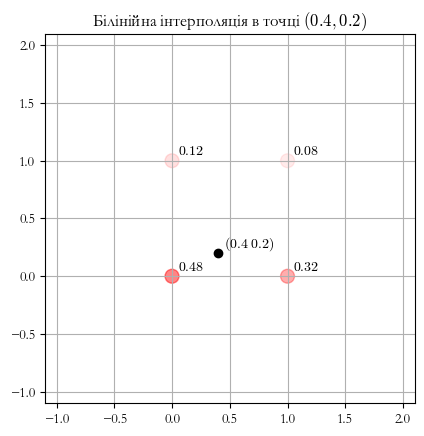
\includegraphics[width=0.5\textwidth]{img/bilinear-interpolation-1.png}
    \caption{
        Візуалізована білінійна інтерполяція в точці $(0{,}4,0{,}2)$ згідно формули~\eqref{e:blinterp}. 
        Значення в дробовій точці утворюється лінійною комбінацією значень у червоних точках на ґратці
        з коефіцієнтами, вказаними над точками.
    }
    \label{fig:bilinear-interp}
\end{figure}

Ідея статистики LBP \cite{ojala2002} полягає у використанні малої кількості тестових точок навколо пікселя для грубого опису поведінки його околу.
Побудуємо його з деяких простих міркувань.
Нехай все наше зображення містить лише одну текстуру.
У загальному випадку, статистика $T \colon K \to \R$ --- це скалярна функція, визначена для кожного пікселя зображення. 
При цьому, нехай $N_c \subset K$ --- множина координат пікселів, від значень яких залежить значення $T(c)$, $c \in K$. 
Вважатимемо, що $N_c$ будується для кожного пікселя однаково, на основі множини зсувів $R = \{r_i\} \subset \R^2$, $N_c = \{c' \mid c' - c \in R\}$, $0 = r_0 \in R$.
Тоді $T(c) = T(g_0, g_1, g_2, \dots, g_n)$, де $g_i = I(c_i)$, $c_i \in N_c$, при чому $g_0 = I(c)$, $\# N_c = n+1$.

LBP побудований в першу чергу з міркувань інваріантності відносно контрастності зображення.
Також, емпірично відомо, що значення ``центрального'' пікселя несе мало інформації, а важливішими є відносні значення рівнів.  
Зміна контрастності зображення математично описується монотонним перетворенням значень його пікселів: $I' = G \circ I$, $G \colon [0,255] \to [0,255]$, де $G$ -- строго монотонна.
В такому разі, вимагаємо $T(g_0, g_1, \dots , g_n) = T(G(g_0), G(g_1), \dots , G(g_n))$.
Одне з допустимих визначень має вигляд $T = T(\{s(g_i - g_j) \mid 0\le i<j \le n\})$, де $s(x) = \1(x \ge 0)$.
Нехтуючи значенням центрального пікселя і відносними рівнями інших пікселів, можна спростити його до $T = T(\{s(g_i - g_0) \mid i=\overline{1,n}\})$.

Найповніший опис околу за таких умов був би самим бінарним вектором $\tilde T(c) \in \{0,1\}^n$,
де $\tilde T(c)_k = s(g_k - g_0)$, $k=\overline{1,n}$.
Бінарні вектори незручні у використанні у явному вигляді для комп'ютеризованих обчислень, проте, трактуючи їх як двійковий запис деякого числа, 
їх можна ототожнити із цілими числами. Математично така статистика формулюється як 
\begin{equation}\label{e:ojala-T}
    T(c) = T(s(g_1 - g_0), s(g_2 - g_0), \dots , s(g_n - g_0)) = \sum_{k=1}^n 2^{k-1}s(g_k-g_0),
\end{equation}

Перейдемо до питання побудови околу $N_c$. 
Наразі статистика $T$ не є інваріантною відносно обертання, проте необхідною умовою для цього є розташування тестових точок $c_1,\dots ,c_n$ у 
радіальній симетрії відносно центру $c$.
Через скінченну роздільну здатність зображення було би недоцільно розглядати симетрію відносно повороту на довільно малий кут.
Тому, прийнято дискретизувати простір кутів на $P$ значень і розглядати симетрію лише відносно поворотів на кути кратні $\frac{2\pi}{P}$.
Ціле число $P$ називатимемо \emph{рівнем дискретизації}, а $\frac{2\pi}{P}$ -- \emph{кутом дискретизації}. 

У загальному випадку, тестові точки $N_c$ можуть бути розташовані на колах різних радіусів. 
На практиці прийнято розділяти точки різних радіусів на різні околи, тому вважатимемо, що усі точки $c_1,\dots ,c_n$ лежать на одному колі радіуса $R$.
Звідси, маємо, що всі точки мають бути рівномірно розподілені по колу з кроком, сумісним із $\frac{2\pi}{P}$.
Для визначенності, першу точку $c_1$ прийнято ставити праворуч від центру, за кутом 0 відносно горизонтальної осі, а наступні нумерувати за збільшенням кута.

Найчастіше, радіальний окіл $N_c$ радіуса $R$ та дискретизації $P$ має рівно $P$ точок і визначається як
\begin{equation}\label{e:circle}
    c_k = c_0 + R \cdot \begin{pmatrix} \cos \frac{2\pi (k-1)}{P} & \sin \frac{2\pi (k-1)}{P} \end{pmatrix}, \quad k=\overline{1,P}
\end{equation}
Зауважу, що точки околу переважно мають дробові координати, тобто значення $I(c_k)$ мають обчислюватися шляхом білінійної інтерполяції за формулою~\eqref{e:blinterp}.

\begin{figure}[h]
    \begin{subfigure}{0.48\textwidth}
    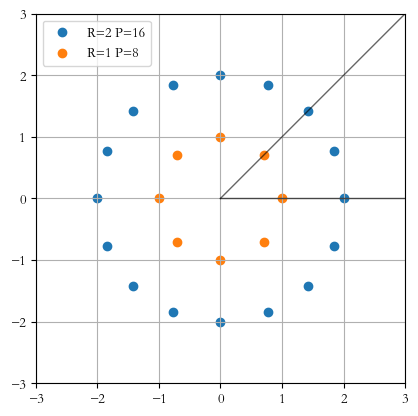
\includegraphics[width=0.9\linewidth]{img/clique-2.png} 
    \caption{
        Типовий окіл для обчислення інваріантної відносно обертання статистики із дискретизацією 8 або $\frac{\pi}{4}$. 
    }
    \label{subfig:clique-2a}
    \end{subfigure}%
    \hfill
    \begin{subfigure}{0.48\textwidth}
    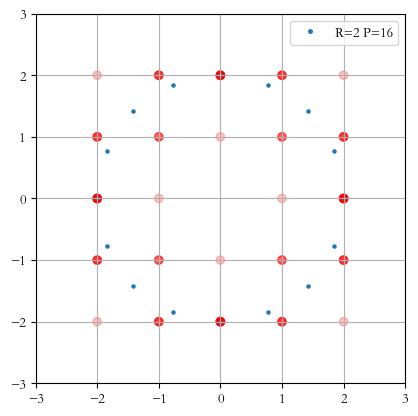
\includegraphics[width=0.9\linewidth]{img/clique-2-interp.png}
    \caption{
        Фактичні точки на ґратці, що приймають участь у обчисленні статистики на околі радіуса 2.
    }
    \label{subfig:clique-2b}
    \end{subfigure}
    
    \caption{}
    \label{fig:clique-2}
\end{figure}

\subsection{Узагальнений \(\mathrm{LBP}_{R,P}\)}\label{section1.1a}\hfill

Узагальнені LBP коди \cite{ojala2002} визначаються в точності згідно формули~\eqref{e:ojala-T} на околі~\eqref{e:circle}, покладаючи $n=P$.
При цьому $R$ та $P$ є гіперпараметрами, підбір яких є нетривіальною задачею.
Поширено використання векторної статистики $T = \begin{pmatrix}
    \mathrm{LBP}_{R_1,P_1} & \dots  & \mathrm{LBP}_{R_m,P_m}
\end{pmatrix}$. В такому випадку, $P$ може однозначно залежати від $R$ \cite{fastlbp2024}, або залишатись сталим для всіх радіусів \cite{huawudeng2004}.
За параметрів $R=1$, $P=8$ ми отримуємо статистику, близьку до першої версії статистики локальних бінарних шаблонів $\mathrm{LBP}_8$, у якій окіл визначається не на колі, а на 8-ми сусідніх пікселях.

На практиці, значення $P$ не може необмежено зростати: після $P=64$ числові значення $T$ виходять за межі діапазону значень типової цілочисленої змінної сучасних комп'ютерів довжиною в 64 біти, 
що робить околи більших розмірів недоцільними. У таких випадках доцільно розбивати більші околи на декілька менших, і працювати з вектором статистик відповідних околів,
що грубо відповідатиме конкатенації бітових векторів. 

На основі цього текстурного дескриптора часто будують інші, деякі з них перелічені далі.
Достатньо мале $P$ також означає, що похідний дескриптор $T' = F \circ T$ доцільно реалізовувати з допомогою обчислених заздалегідь таблиці пошуку у вигляді масиву, 
де індексами будуть можливі значення $T$.
Тоді, обчисленя $T'$ зводиться до обчислення $T$ та отримання значення цього масиву за індексом $T$, що часто є набагато швидшою операцією, ніж обчислення $T'$.
Розмір таблиці пошуку залежить від області визначення похідного дескриптора; 
для $F \colon \{\overline{0,2^P}\} \to \{\overline{0,2^P}\}$ та $P\le 64$ таблиця складатиметься з цілочисленних значень не більш, ніж int64, 
а отже матиме розмір $W_P$ не більше ніж $W_P = 2^P \cdot 8$ байтів. 
Для прикладу, $W_{32} \approx 34{,}3$ GB, що є непрактичним обсягом пам'яті, але $W_{24} \approx 135$ MB і $W_{16} \approx 0{,}5$ MB.

\subsection{Інваріантність відносно обертання у \(\mathrm{LBP}_{R,P}^{ri}\)}\label{section1.1c}\hfill

В основному, текстурні дескриптори розробляються у припущенні, що орієнтація текстур у тренувальних та тестових зображеннях співпадають.
Якщо орієнтація текстур довільна, то якість класифікації на основі цих дескрипторів стрімко падає. 
Очевидним рішенням буде доповнювати тренувальні дані синтетичними зображеннями, утвореними обертанням оригінальних. 
Іншим підходом буде використовувати в побудові дескриптора інваріантні статистики (напр. інваріантний LBP) чи 
``стерти" інформацію про орієнтацію зі статистик чи з дескриптора (напр. з допомогою DFT). 
На практиці, точність класифікації суттєво покращується при перетворенні варіантних ознак на комбінацію інваріантних ознак, та ознак із інформацію про орієнтацію, наприклад з допомогою фільтрів Габора \cite{guo2010lbpv}. 

Нехай $\operatorname{rot} : \{0,1\}^P \to \{0,1\}^P$, 
$\operatorname{rot} \begin{pmatrix}a_1 & a_2 & \dots  & a_P\end{pmatrix} = \begin{pmatrix}a_P & a_1 & \dots  & a_{P-1}\end{pmatrix}$ 
--- оператор циклічної перестановки елементів вектора.
Введемо відношення еквівалентності $A\sim B \iff \exists k: A = \operatorname{rot}^k B$, де $A,B \in \{0,1\}^P$.
Зверну увагу, що $\operatorname{rot}^P A = A$ та $\operatorname{rot}^{P-k} \operatorname{rot}^k A = A$.

За цим відношенням еквівалентності розіб'ємо простір значень бінарного вектора $A = \begin{pmatrix}
    s(g_1 - g_0) & s(g_2 - g_0) & \dots  & s(g_P - g_0)
\end{pmatrix}$, з якого далі обчислюється статистика $\mathrm{LBP}_{R,P}$. 
Циклічна перестановка цього вектора відповідає циклічній перестановці індексів точок $c_1, c_2, \dots , c_P$ околу навколо $c_0$, визначеного у~\eqref{e:circle} 
(що у свою чергу моделює обертання зображення на кут, кратний куту дискретизації).
Інваріантний відносно обертання дескриптор $\mathrm{LBP}^{ri}$ обчислюється як найменше числове значення $\mathrm{LBP}_{R,P}$ серед таких околів,
тобто найменше числове значення серед циклічних перестановок бінарного вектора $A \in \{0,1\}^P$,
\begin{equation*}
    \mathrm{LBP}^{ri}_{R,P} = \min_{0\le k < P} \mathrm{LBP}_{R,P} \left( \operatorname{rot}^k A \right).
    % = \min_{0\le k < P} \sum_{i=1}^P s(g_{(i + k) \operatorname{mod} P} - g_0) 2^{(i + k - 1) \operatorname{mod} P}.
\end{equation*}
Ця величина також називається (лексикографічно) мінімальним обертанням рядка $A$ або словом Ліндона.   

Окрім набуття інваріантності, оператор $\mathrm{LBP}^{ri}_{R,P}$ також має меншу область значень, ніж $\mathrm{LBP}_{R,P}$.
Позначимо клас еквівалентності $A$ за відношенням еквівалентності, породженим прообразом $\mathrm{LBP}^{ri}_{R,P}$, як $[A]$.
Тобто, $A \sim A' \iff \mathrm{LBP}^{ri}_{R,P} A = \mathrm{LBP}^{ri}_{R,P} A'$.
Розмір класів еквівалнетності не сталий і залежить від періоду вектора. 
Наприклад, $\# [\texttt{00000000}] = 1$, $\# [\texttt{01010101}] = \# \{01010101,10101010\} = 2$, $\# [00100100] = 8$.

Назвемо вектор періодичним з періодом $0<k\le P$, якщо $\operatorname{rot}^k A = A$ і $k$ є найменшим таким числом.
Вектор з періодом $P$ назвемо неперіодичним.
Зауважу, що не всі періоди можливі. Нехай $d=\operatorname{gcd}(k,P)$ -- найбільше спільне кратне, $d\le k < P$. 
Існують $r,s\in \Z$ такі, що $d=rk+sP$. Тоді $\operatorname{rot}^d A = \operatorname{rot}^{rk+sP} A = \operatorname{rot}^{rk} A = A$.
Але $k$ -- найменше таке число, тобто $k \le d$, звідки маємо $d=k$. Таким чином, періоди -- це дільники $P$.
Зрозуміло, що клас еквівалентності $k$-періодичного вектора тоді має розмір $k$, проте кількість різних $k$-періодичних векторів нетривіальна.
Проте, зрозуміло, що $\# \{A\in \{0,1\}^P \mid \operatorname{rot}^k A = A\} = \operatorname{gcd}(k,P)$.  

Тоді, за лемою Бернсайда, $\mathrm{LBP}^{ri}_{R,P}$ приймає $N^{ri}_P = \frac{1}{P}\sum_{k=1}^P 2^{\operatorname{gcd}(k,P)}$ різних значень. 
Ця величина природним чином є кількістю різних орбіт дії групи $\Z/P\Z$ на $\{0,1\}^P$, а також, кількістю різних двоколірних намист довжини $P$.
Асимптотично, $N^{ri}_P \sim \frac{2^P}{P} + o(2^P)$. 
Для прикладу, $N^{ri}_8 = 36$, $N^{ri}_{16} = 4116$, $N^{ri}_{24} = 699252$

\subsection{Рівномірний \(\mathrm{LBP}_{R,P}^{riu}\) та інші}\label{section1.1d}\hfill

У подальших дослідженнях \cite{ojala2002} було помічено, що для деяких застосувань та малих радіусів найчастіше (90\% та більше) трапляються так звані ``рівномірні'' (uniform) послідовності, 
в яких є чітка межа між одиницями та нулями, тобто не більш ніж 2 переходи від 0 до 1 чи назад. 
Тобто, мінімальне представлення бінарного вектору $A$ матиме $u$ нулів, за якими йдуть $P-u$ одиниць.
Після цього спостереження розроблено ``рівномірний'' $\mathrm{LBP}^{riu}_{R,P}$, 
який ставить у відповідність рівномірному вектору кількість одиниць від $0$ до $P$, а нерівномірному -- спеціальне значення $P+1$.
$\mathrm{LBP}^{riu}_{R,P}$ приймає $P+2$ різних значень.

Наше дослідження \cite{fastlbp2024} базується на доробку Benjamin Woodhams, долученого до \cite{lee2025integrated}, і використовує саме цей варіант дескриптора LBP.
Його доцільність залишається дискусійним питанням, бо у випадку великих зображень та великих радіусів 
частка рівномірних околів стрімко зменшується.

\begin{figure}[h]
    \centering
    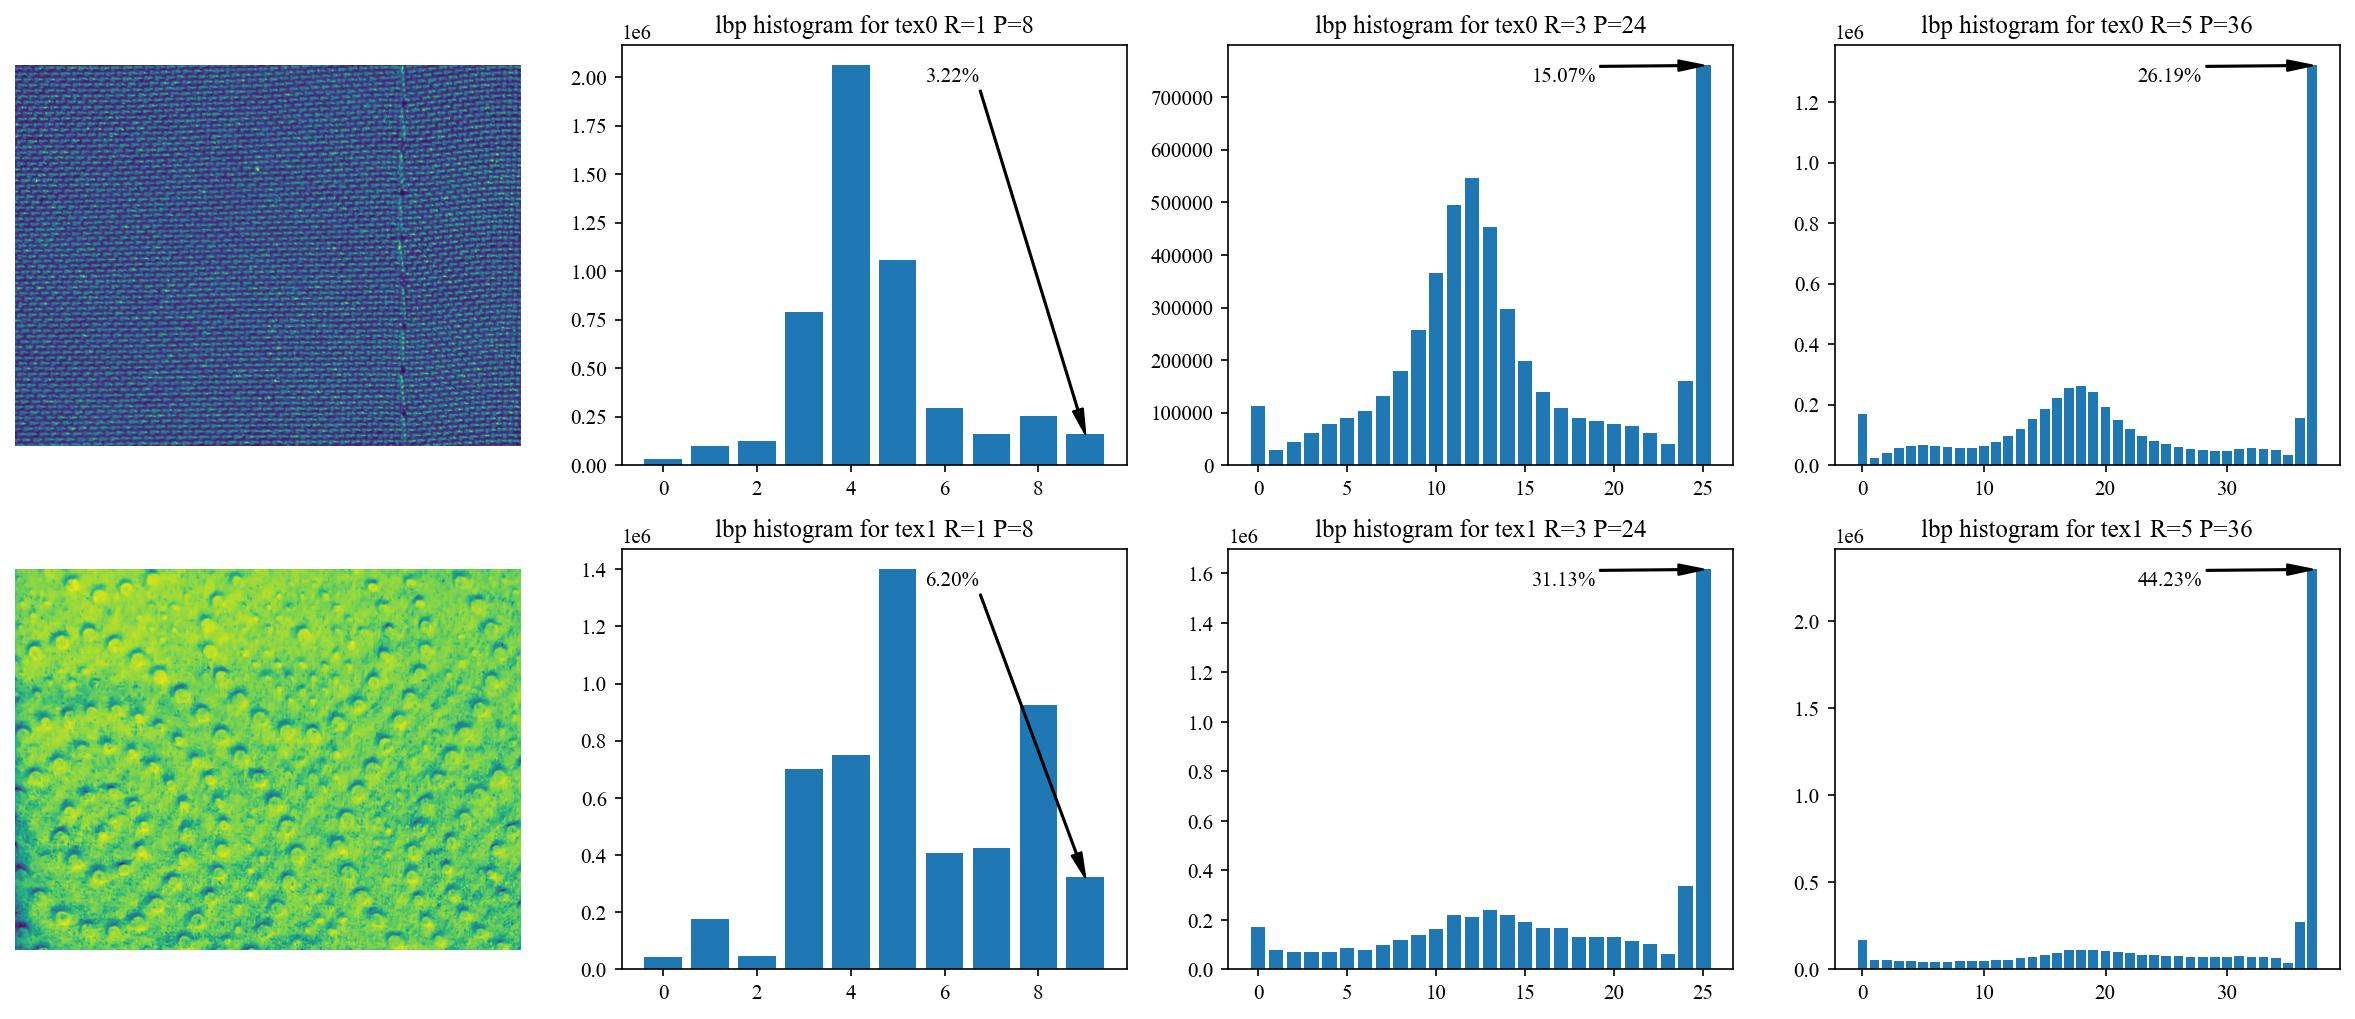
\includegraphics[width=0.99\textwidth]{img/cloth-hist-lbpu.jpg}
    \caption{
        Гістограми LBP із різними $R$ та $P$ для двох текстур.
        Демонструється збільшення кількості нерівномірних околів зі збільшенням R.
    }
    \label{fig:cloth-hist-lbpu}
\end{figure}

Інший цікавий підхід полгає у застосуванні амплітуди дискретного перетворення Фур'є (DFT) LBP кодів у якості ознак \cite{arof1998, haley1999}.
Відомо, що DFT вектора не змінюється від його циклічних перестановок. 
Більше того, через симетричність амплітуди DFT відносно середини послідовності, достатньо зберігати лише половину координат, що зменшує кількість ознак. 

% =============================================
